%DIF 1-4d1
%DIF LATEXDIFF DIFFERENCE FILE
%DIF DEL gmc.tex      Wed Aug 19 22:03:15 2026
%DIF ADD gmc_v1.tex   Sat Aug 22 16:26:42 2026
%DIF < % SUPERSEDED 2026-08-19 — the live working file is now 2027_ICASSP/gmc_v1.tex.
%DIF < % Keep this one for comparison only; do not edit. Content corrections to the live
%DIF < % file are tracked in issues #23 (numeric/factual) and #24 (narrative).
%DIF < %
%DIF -------
% Template for ICASSP-2024 paper; to be used with:
%          spconf.sty  - ICASSP/ICIP LaTeX style file, and
%          IEEEbib.bst - IEEE bibliography style file.
% --------------------------------------------------------------------------
\documentclass{article}
\usepackage{spconf,amsmath,graphicx}
\usepackage{multirow}              % per-host recipe table
\usepackage{microtype}             % kills sub-3pt overfull, polishes justification
%DIF 13-14d9
%DIF < \usepackage{tikz}                  % Fig 1 pipeline + Fig 2 ego-motion schematic (self-contained, no asset)
%DIF < \usetikzlibrary{arrows.meta,positioning,fit,backgrounds}
%DIF -------
\usepackage{csquotes}
\usepackage{comment}
%DIF 17a11
\usepackage{xcolor} %DIF > 
%DIF -------

% Example definitions.
% --------------------
\def\x{{\mathbf x}}
\def\L{{\cal L}}

% Title.
% ------
\title{Referring Multi-Object Tracking in Moving-Camera Videos via Global Motion Compensation}
%
% Single address.
% ---------------
\name{Author(s) Name(s)}
\address{Author Affiliation(s)}
%
% For example:
% ------------
%\address{School\\
%	Department\\
%	Address}
%
% Two addresses (uncomment and modify for two-address case).
% ----------------------------------------------------------
%\twoauthors
%  {A. Author-one, B. Author-two\sthanks{Thanks to XYZ agency for funding.}}
%	{School A-B\\
%	Department A-B\\
%	Address A-B}
%  {C. Author-three, D. Author-four\sthanks{The fourth author performed the work
%	while at ...}}
%	{School C-D\\
%	Department C-D\\
%	Address C-D}
%
%DIF PREAMBLE EXTENSION ADDED BY LATEXDIFF
%DIF UNDERLINE PREAMBLE %DIF PREAMBLE
\RequirePackage[normalem]{ulem} %DIF PREAMBLE
\RequirePackage{color}\definecolor{RED}{rgb}{1,0,0}\definecolor{BLUE}{rgb}{0,0,1} %DIF PREAMBLE
\providecommand{\DIFadd}[1]{{\protect\color{blue}\uwave{#1}}} %DIF PREAMBLE
\providecommand{\DIFdel}[1]{{\protect\color{red}\sout{#1}}} %DIF PREAMBLE
%DIF SAFE PREAMBLE %DIF PREAMBLE
\providecommand{\DIFaddbegin}{} %DIF PREAMBLE
\providecommand{\DIFaddend}{} %DIF PREAMBLE
\providecommand{\DIFdelbegin}{} %DIF PREAMBLE
\providecommand{\DIFdelend}{} %DIF PREAMBLE
\providecommand{\DIFmodbegin}{} %DIF PREAMBLE
\providecommand{\DIFmodend}{} %DIF PREAMBLE
%DIF FLOATSAFE PREAMBLE %DIF PREAMBLE
\providecommand{\DIFaddFL}[1]{\DIFadd{#1}} %DIF PREAMBLE
\providecommand{\DIFdelFL}[1]{\DIFdel{#1}} %DIF PREAMBLE
\providecommand{\DIFaddbeginFL}{} %DIF PREAMBLE
\providecommand{\DIFaddendFL}{} %DIF PREAMBLE
\providecommand{\DIFdelbeginFL}{} %DIF PREAMBLE
\providecommand{\DIFdelendFL}{} %DIF PREAMBLE
\providecommand{\DIFscaledelfig}{0.5}
%DIF HIGHLIGHTGRAPHICS PREAMBLE %DIF PREAMBLE
\RequirePackage{settobox} %DIF PREAMBLE
\RequirePackage{letltxmacro} %DIF PREAMBLE
\newsavebox{\DIFdelgraphicsbox} %DIF PREAMBLE
\newlength{\DIFdelgraphicswidth} %DIF PREAMBLE
\newlength{\DIFdelgraphicsheight} %DIF PREAMBLE
% store original definition of \includegraphics %DIF PREAMBLE
\LetLtxMacro{\DIFOincludegraphics}{\includegraphics} %DIF PREAMBLE
\providecommand{\DIFaddincludegraphics}[2][]{{\color{blue}\fbox{\DIFOincludegraphics[#1]{#2}}}} %DIF PREAMBLE
\providecommand{\DIFdelincludegraphics}[2][]{% %DIF PREAMBLE
\sbox{\DIFdelgraphicsbox}{\DIFOincludegraphics[#1]{#2}}% %DIF PREAMBLE
\settoboxwidth{\DIFdelgraphicswidth}{\DIFdelgraphicsbox} %DIF PREAMBLE
\settoboxtotalheight{\DIFdelgraphicsheight}{\DIFdelgraphicsbox} %DIF PREAMBLE
\scalebox{\DIFscaledelfig}{% %DIF PREAMBLE
\parbox[b]{\DIFdelgraphicswidth}{\usebox{\DIFdelgraphicsbox}\\[-\baselineskip] \rule{\DIFdelgraphicswidth}{0em}}\llap{\resizebox{\DIFdelgraphicswidth}{\DIFdelgraphicsheight}{% %DIF PREAMBLE
\setlength{\unitlength}{\DIFdelgraphicswidth}% %DIF PREAMBLE
\begin{picture}(1,1)% %DIF PREAMBLE
\thicklines\linethickness{2pt} %DIF PREAMBLE
{\color[rgb]{1,0,0}\put(0,0){\framebox(1,1){}}}% %DIF PREAMBLE
{\color[rgb]{1,0,0}\put(0,0){\line( 1,1){1}}}% %DIF PREAMBLE
{\color[rgb]{1,0,0}\put(0,1){\line(1,-1){1}}}% %DIF PREAMBLE
\end{picture}% %DIF PREAMBLE
}\hspace*{3pt}}} %DIF PREAMBLE
} %DIF PREAMBLE
\LetLtxMacro{\DIFOaddbegin}{\DIFaddbegin} %DIF PREAMBLE
\LetLtxMacro{\DIFOaddend}{\DIFaddend} %DIF PREAMBLE
\LetLtxMacro{\DIFOdelbegin}{\DIFdelbegin} %DIF PREAMBLE
\LetLtxMacro{\DIFOdelend}{\DIFdelend} %DIF PREAMBLE
\DeclareRobustCommand{\DIFaddbegin}{\DIFOaddbegin \let\includegraphics\DIFaddincludegraphics} %DIF PREAMBLE
\DeclareRobustCommand{\DIFaddend}{\DIFOaddend \let\includegraphics\DIFOincludegraphics} %DIF PREAMBLE
\DeclareRobustCommand{\DIFdelbegin}{\DIFOdelbegin \let\includegraphics\DIFdelincludegraphics} %DIF PREAMBLE
\DeclareRobustCommand{\DIFdelend}{\DIFOaddend \let\includegraphics\DIFOincludegraphics} %DIF PREAMBLE
\LetLtxMacro{\DIFOaddbeginFL}{\DIFaddbeginFL} %DIF PREAMBLE
\LetLtxMacro{\DIFOaddendFL}{\DIFaddendFL} %DIF PREAMBLE
\LetLtxMacro{\DIFOdelbeginFL}{\DIFdelbeginFL} %DIF PREAMBLE
\LetLtxMacro{\DIFOdelendFL}{\DIFdelendFL} %DIF PREAMBLE
\DeclareRobustCommand{\DIFaddbeginFL}{\DIFOaddbeginFL \let\includegraphics\DIFaddincludegraphics} %DIF PREAMBLE
\DeclareRobustCommand{\DIFaddendFL}{\DIFOaddendFL \let\includegraphics\DIFOincludegraphics} %DIF PREAMBLE
\DeclareRobustCommand{\DIFdelbeginFL}{\DIFOdelbeginFL \let\includegraphics\DIFdelincludegraphics} %DIF PREAMBLE
\DeclareRobustCommand{\DIFdelendFL}{\DIFOaddendFL \let\includegraphics\DIFOincludegraphics} %DIF PREAMBLE
%DIF AMSMATHULEM PREAMBLE %DIF PREAMBLE
\makeatletter %DIF PREAMBLE
\let\sout@orig\sout %DIF PREAMBLE
\renewcommand{\sout}[1]{\ifmmode\text{\sout@orig{\ensuremath{#1}}}\else\sout@orig{#1}\fi} %DIF PREAMBLE
\makeatother %DIF PREAMBLE
%DIF COLORLISTINGS PREAMBLE %DIF PREAMBLE
\RequirePackage{listings} %DIF PREAMBLE
\RequirePackage{color} %DIF PREAMBLE
\lstdefinelanguage{DIFcode}{ %DIF PREAMBLE
%DIF DIFCODE_UNDERLINE %DIF PREAMBLE
  moredelim=[il][\color{red}\sout]{\%DIF\ <\ }, %DIF PREAMBLE
  moredelim=[il][\color{blue}\uwave]{\%DIF\ >\ } %DIF PREAMBLE
} %DIF PREAMBLE
\lstdefinestyle{DIFverbatimstyle}{ %DIF PREAMBLE
	language=DIFcode, %DIF PREAMBLE
	basicstyle=\ttfamily, %DIF PREAMBLE
	columns=fullflexible, %DIF PREAMBLE
	keepspaces=true %DIF PREAMBLE
} %DIF PREAMBLE
\lstnewenvironment{DIFverbatim}[1][]{\lstset{style=DIFverbatimstyle}}{} %DIF PREAMBLE
\lstnewenvironment{DIFverbatim*}[1][]{\lstset{style=DIFverbatimstyle,showspaces=true}}{} %DIF PREAMBLE
\lstset{extendedchars=\true,inputencoding=utf8}

%DIF END PREAMBLE EXTENSION ADDED BY LATEXDIFF

\begin{document}
%DIF < \ninept
\DIFaddbegin \ninept
\DIFaddend %
\maketitle
%
\begin{abstract}
  Referring multi-object tracking (RMOT) takes a video and a natural-language expression as input and tracks all objects described by the expression. Many expressions describe how an object moves rather than how it appears. In a video captured by moving cameras, a parked vehicle may appear to move, while a vehicle moving with the camera may show little displacement. Existing motion-language RMOT methods align motion with text but do not explicitly remove camera-induced motion. In this paper, we propose extracting residual motion across frames \DIFaddbegin \DIFadd{\textcolor{red}{by estimating camera motion from road-region background correspondences in driver-view videos} }\DIFaddend and comparing motion features with the query language expression. We consider the motion-matching extent and integrate it with the RMOT method's prediction result \DIFaddbegin \DIFadd{\textcolor{red}{through late fusion with host-specific weights}}\DIFaddend . In the evaluation, we verify the performance gain by taking the proposed motion compensation module as a plug-in \DIFdelbegin \DIFdel{. 
%DIF < On iKUN~\cite{ikun}, GMC-Link improves moving-class Higher Order Tracking Accuracy (HOTA)~\cite{hota} from $25.53$ to $29.95$, corresponding to a gain of $4.42$ points over five random seeds. Ego-motion compensation contributes $2.12$ moving-class HOTA ($p{<}10^{-3}$) and $0.71$ static-class HOTA ($p{<}10^{-3}$) over raw image-plane motion. These results show that compensation helps both recover truly moving objects and reject stationary objects affected by camera motion. Across the three evaluated host--split settings, larger gains are observed for hosts with lower native moving-class HOTA. In pooled HOTA, GMC-Link stays within seed noise of the published iKUN result and improves FlexHook~\cite{flexhook} on Refer-KITTI V2~\cite{temprmot} by $0.158$, while FlexHook on Refer-KITTI V1~\cite{transrmot} remains below its published score because of a known reproduction gap. 
}\DIFdelend \DIFaddbegin \DIFadd{\textcolor{red}{across different RMOT hosts. On iKUN, the module raises moving-class HOTA by $7.08$ points, and all three evaluated settings exceed their hosts' published pooled HOTA}.
}\DIFaddend \end{abstract}
%
\begin{keywords}
  referring multi-object tracking, ego-motion compensation, motion-language alignment, plug-in module, Refer-KITTI, video grounding
\end{keywords}

%-------------------------------

\section{Introduction}
\label{sec:intro}
Referring multi-object tracking (RMOT) outputs tracking results of the objects described by a free-form language expression. For example, a \enquote{left-vehicles-in-red} description targets the red vehicles on the left. However, many descriptions focus on object motion, such as \enquote{moving cars} or \enquote{a vehicle turning left}. In videos captured by a moving camera, the observed motion is a mixture of object motion and camera motion, and thus a static car may appear to move, while a moving car may appear static across video frames.

Previous RMOT methods~\cite{transrmot,ikun,flexhook} match language expressions to objects.  VMRMOT~\cite{vmrmot} considers explicit motion cues, such as changes in direction and speed, in the matching process. All of these methods, however, compute motion from the object's bounding-box displacement across frames, which mixes object motion with camera motion in a video captured by moving cameras.

Conventional multi-object tracking (MOT) methods already proposed to remove camera motion: BoT-SORT~\cite{botsort} estimates camera-induced image motion, while UCMCTrack~\cite{ucmctrack} stabilizes object trajectories. How motion compensation can be extended to RMOT is still underexplored.

%However, the compensated motion never reaches the language-matching stage. Camera motion could in principle be obtained from the global positioning system (GPS) and inertial measurement unit (IMU) recordings provided by KITTI~\cite{kitti}, which Refer-KITTI is built on. These sensors measure the position and orientation of the recording vehicle in the world, not how the camera's movement shifts pixels in the video. Converting between the two requires additional information: the pixel shift produced by a given camera movement depends on the camera's focal length, its mounting on the vehicle, and each point's distance from the camera. Moreover, general videos do not come with GPS or IMU recordings. We therefore estimate camera motion directly from image features, which keeps the module self-contained: it consumes only the frames the host model already uses and can be attached to different two-stage RMOT frameworks without modifying their architectures.

We propose separating camera motion from object motion and providing motion information for language-guided tracking. It consists of four stages. First, a homography, which describes the geometric transformation across frames, is estimated to measure camera motion. The estimated homographies are accumulated across frames to reliably measure object motion. Second, residual velocity, which represents object motion after removing camera motion, is computed across frames and used as a temporal motion feature. Third, a Contrastive Motion Aligner is developed to compare motion features with language expressions and produce a motion-matching score. Finally, the motion-matching score is \DIFdelbegin \DIFdel{scaled by a single host-specific weight }\DIFdelend \DIFaddbegin \DIFadd{\textcolor{red}{scaled by a host-specific weight} }\DIFaddend and added to the host's matching score. Here, the host model refers to a two-stage RMOT method we use as a baseline, such as iKUN~\cite{ikun} and FlexHook~\cite{flexhook}. The proposed process is taken as a plug-in to provide an extra motion-matching score. We thus improve existing RMOT baselines without retraining them.

The accumulated homographies are the key component. By compensating for camera motion, they allow the motion feature to better represent the object's actual movement rather than the apparent motion induced by camera movement. They also preserve motion information across frames, enabling the model to capture motion patterns described by expressions such as \enquote{moving} or \enquote{turning}.

%This design leads to a two-sided prediction that can be tested directly: if residual velocity is replaced with raw image velocity, moving-class accuracy should decrease because objects travelling with the camera lose their image displacement, and static-class accuracy should also decrease because parked objects inherit the camera's motion. Section~\ref{sec:exp} confirms both effects and shows that, among the module's design choices, camera motion compensation is the only one whose removal significantly degrades either class. Compensation therefore makes the motion feature effective for object disambiguation rather than simply providing additional motion cues.

This work connects ego-motion compensation with motion-language modeling for RMOT. Our main contributions are as follows.
\begin{itemize}
  \item We propose a plug-in that aligns ego-compensated residual velocity with the referring expression, thereby improving the host RMOT method without modifying or retraining it.
        %  \item We show that among the module's design choices, camera motion compensation is the key factor: it is the only component whose removal significantly degrades both moving-class ($p{=}0.006$) and static-class ($p{<}10^{-4}$) HOTA.
  \item \DIFdelbegin \DIFdel{Based on iKUN, the proposed plug-in raises moving-class HOTA by $4.69$. The performance gains can be observed in various settings.
}\DIFdelend \DIFaddbegin \DIFadd{\textcolor{red}{Across iKUN and FlexHook, GMC-Link improves pooled HOTA in all three evaluated host settings. On iKUN, it raises MOVING HOTA from $25.531$ to $32.606\pm0.654$ (approximately $+7.08$ points).}
}\DIFaddend \end{itemize}

%---------------------

\begin{figure*}
  \centering
  \DIFdelbeginFL %DIFDELCMD < 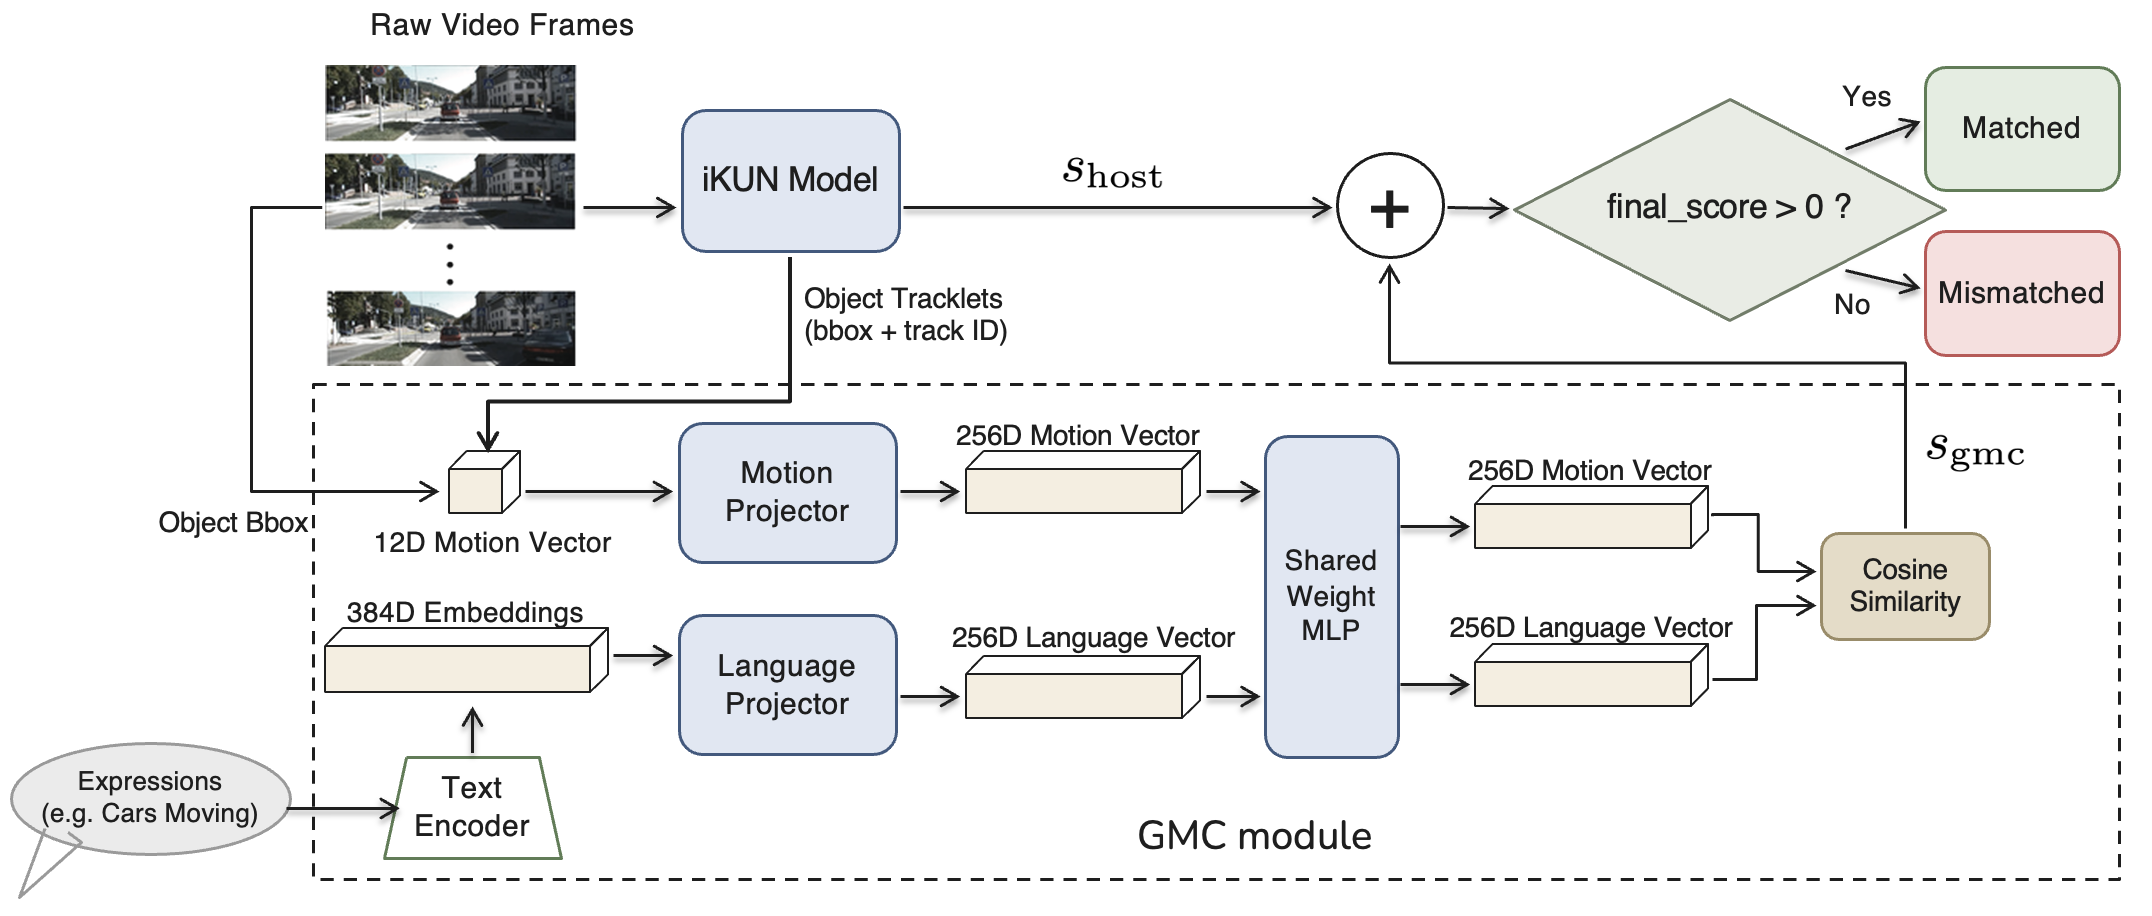
\includegraphics[width=14cm]{figures/Architecture.png}
%DIFDELCMD < %%%
\DIFdelendFL \DIFaddbeginFL 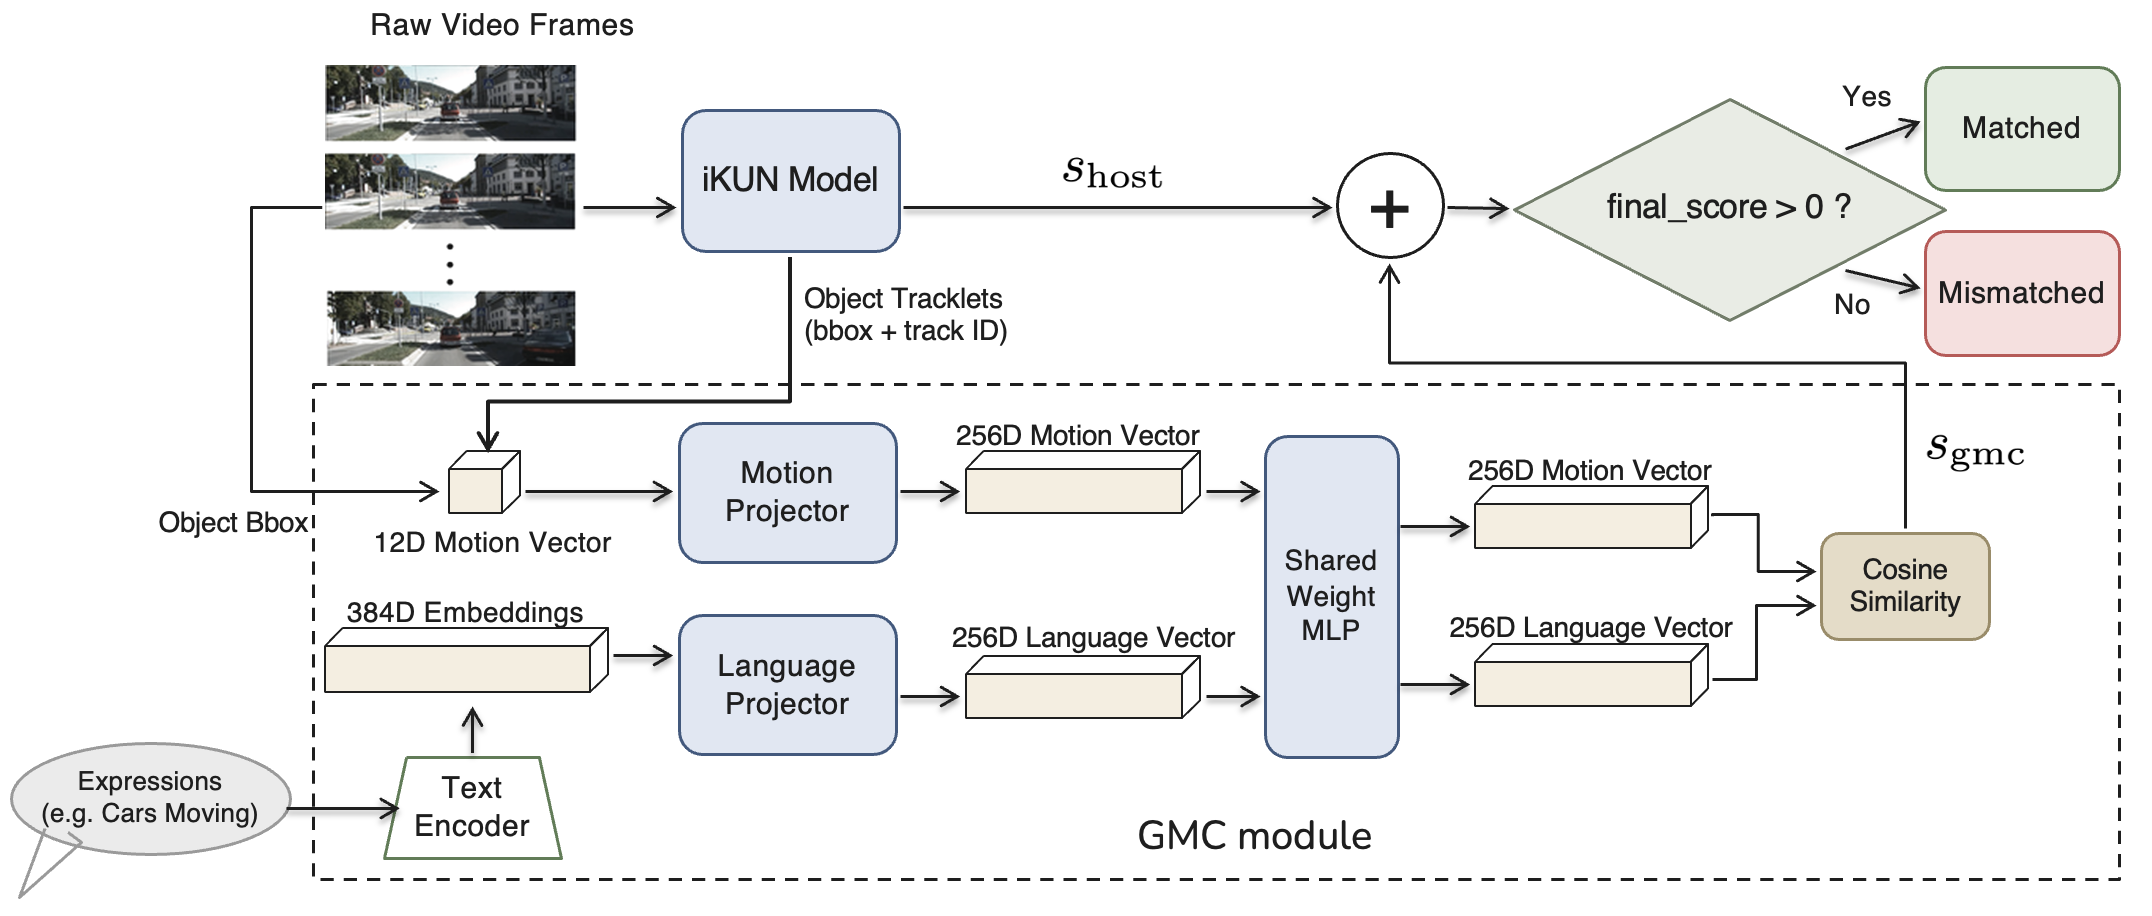
\includegraphics[width=12cm]{figures/Architecture.png}
  \DIFaddendFL \caption{The host model, iKUN in this case, provides tracking scores. The GMC-Link estimates camera motion, derives residual motion, aligns it with language, and provides an extra cue to adjust the tracking scores.}
  \label{fig:architecture}
\end{figure*}

\section{Related Works}
\label{sec:related}
\subsection{Referring MOT and motion-language fusion}
TransRMOT~\cite{transrmot} introduced the RMOT task on the Refer-KITTI dataset. Later methods improved different parts of this task. iKUN~\cite{ikun} separated language-based object matching from object tracking, while FlexHook~\cite{flexhook} improved how visual and language information interact. ReferGPT~\cite{refergpt} used a multimodal large language model to describe existing object tracks, and MEX~\cite{mex} provided a memory-efficient module for matching tracks with language.

\DIFdelbegin \DIFdel{More recent RMOT methods~\mbox{%DIFAUXCMD
\cite{mlstrack,deeprmot,cdrmot,tellmewhat} }\hskip0pt%DIFAUXCMD
further improve models' understanding of object descriptions. }\DIFdelend \DIFaddbegin \DIFadd{\textcolor{red}{More recent RMOT methods~\cite{deeprmot} further improve models' understanding of object descriptions. STORM~\cite{storm} unifies grounding and tracking in an end-to-end multimodal large language model.} }\DIFaddend VMRMOT~\cite{vmrmot} explicitly represents motion using information such as position, direction, changes in distance, and changes in speed. However, these methods still estimate object motion from the object's bounding-box movements across frames. When the camera moves, the observed bounding-box movement contains both object motion and camera motion. %Therefore, a stationary object may appear to be moving, while a moving object may appear nearly stationary. This makes it difficult for the model to correctly understand motion-related expressions.

%TempRMOT~\cite{temprmot} is different because it already stores trajectory history in recurrent memory. In our experiments, adding our external motion module to TempRMOT reduced pooled Higher Order Tracking Accuracy (HOTA) in two separate trials. This result suggests that the additional module may introduce redundant motion information or unnecessary constraints because TempRMOT already models motion over time. We therefore focus on two-stage RMOT models that do not already encode trajectory history in recurrent memory.

\subsection{Camera and ego-motion compensation in tracking}
Camera motion compensation is widely used in traditional multi-object tracking (MOT). BoT-SORT~\cite{botsort} estimates camera-induced motion across frames. UCMCTrack~\cite{ucmctrack} estimates how the camera moves relative to the road surface. EMAP~\cite{emap} further separates the camera's turning and movement from object motion within the Kalman prediction process.

These methods demonstrate that compensating for camera motion can improve tracking objects across frames. However, the compensated positions are mainly used to match objects between adjacent frames. They are not accumulated over time to describe an object's motion, nor are they connected to language expressions. Our method builds on established techniques for separating camera motion from object motion, including plane-plus-parallax analysis~\cite{iranianandan}, homography estimation~\cite{hartleyzisserman}, motion segmentation under moving cameras~\cite{bideau}, and ego-motion estimation in visual odometry~\cite{scaramuzza}. We do not propose a new camera-motion estimation technique. Instead, we convert camera-compensated trajectories into motion features and align them with language for RMOT.

%\subsection{Connecting camera compensation with RMOT}
%Existing RMOT methods can match object motion with language, but their motion estimates are still affected by camera movement. In contrast, camera-compensated MOT removes this effect, but uses the corrected motion only for tracking rather than for language understanding. GMC-Link connects these two research directions. It tracks object motion across multiple frames after removing camera motion, compares this corrected motion with the referring expression, and combines the resulting score with the host model's original score. In this way, the host model keeps its original appearance-based matching ability while gaining additional motion information. 

%------------------------------------


\section{Method}
\label{sec:method}
Figure~\ref{fig:architecture} shows the proposed RMOT framework with the global motion compensation (GMC) module. The GMC module is attached to a two-stage RMOT method, iKUN~\cite{ikun} in this case. iKUN performs object detection and tracking and then outputs appearance-language matching scores. The inputs to the GMC module are the sequence of object bounding boxes across frames, the video frames, and the language expression. Based on these inputs, the GMC module estimates camera motion, extracts residual object motion, aligns it with the language expression, and produces a matching score. The score is then combined with the host model's predicted score, as an embodiment of the late fusion scheme. The \DIFdelbegin \DIFdel{complete pipeline of the GMC module is illustrated in Figure~\ref{fig:pipeline}, which }\DIFdelend \DIFaddbegin \DIFadd{module }\DIFaddend consists of four stages: ego-motion compensation, multi-scale residual velocity extraction, motion-language alignment, and late fusion.


\DIFdelbegin %DIFDELCMD < \begin{figure}
%DIFDELCMD < \centering
%DIFDELCMD < \begin{tikzpicture}[
%DIFDELCMD <   font=\scriptsize,
%DIFDELCMD <   node distance=2.6mm,
%DIFDELCMD <   box/.style={draw, rounded corners, align=center, inner sep=2.5pt,
%DIFDELCMD <               text width=0.55\linewidth, minimum height=5.5mm},
%DIFDELCMD <   sbox/.style={draw, rounded corners, align=center, inner sep=2.5pt, fill=black!4,
%DIFDELCMD <                text width=0.28\linewidth, minimum height=5.5mm},
%DIFDELCMD <   ar/.style={-{Latex[length=1.6mm]}, semithick}
%DIFDELCMD < ]
%DIFDELCMD < \node[box] (frames) {Consecutive frames $I_{t-1},\,I_t$};
%DIFDELCMD < \node[box, below=of frames] (orb) {ORB\,+\,BFMatcher\,+\,RANSAC\\ $\Rightarrow$ frame-to-frame $H_{t-1\to t}$};
%DIFDELCMD < \node[box, below=of orb] (cum) {Compose cumulative $H_{t-k\to t}$;\\ warp original centroids};
%DIFDELCMD < \node[box, below=of cum] (desc) {12D residual velocity\\ gaps $\{2,5,10\}$ + box state};
%DIFDELCMD < \node[box, below=of desc] (align) {Motion-language alignment\\ $\Rightarrow$ cosine score};
%DIFDELCMD < \node[box, below=of align] (fuse) {Additive fusion\\ $s_{\text{host}}+\alpha\, s_{\text{gmc}}$};
%DIFDELCMD < \node[box, below=of fuse] (hota) {Final prediction};
%DIFDELCMD < \node[sbox, right=4mm of align] (text) {Expression\\ $\to$ text encoder 384D};
%DIFDELCMD < \draw[ar] (frames)--(orb);
%DIFDELCMD < \draw[ar] (orb)--(cum);
%DIFDELCMD < \draw[ar] (cum)--(desc);
%DIFDELCMD < \draw[ar] (desc)--(align);
%DIFDELCMD < \draw[ar] (align)--(fuse);
%DIFDELCMD < \draw[ar] (fuse)--(hota);
%DIFDELCMD < \draw[ar] (text)--(align);
%DIFDELCMD < \end{tikzpicture}
%DIFDELCMD < %%%
%DIFDELCMD < \caption{%
{%DIFAUXCMD
\textbf{\DIFdelFL{GMC-Link pipeline.}} %DIFAUXCMD
\DIFdelFL{ORB homographies compose into a cumulative transform, produce a 12D motion feature, align with the expression, and correct the host score through additive fusion.}}
%DIFAUXCMD
%DIFDELCMD < \label{fig:pipeline}
%DIFDELCMD < \end{figure}
%DIFDELCMD < 

%DIFDELCMD < %%%
\DIFdelend \subsection{Ego-motion compensation}
\label{sec:ego}
\DIFdelbegin \DIFdel{This stage estimates camera motion from consecutive video frames so that object motion can be separated from camera-induced motion. We first extract ORB~\mbox{%DIFAUXCMD
\cite{orb} }\hskip0pt%DIFAUXCMD
keypoints from video frames. Keypoints inside objects' bounding boxes are removed so that moving foreground objects do not affect camera-motion estimation. The remaining keypoints at the $(t-1)$-th frame $I_{t-1}$ and the $t$-th frame $I_t$ are matched, and the RANSAC~\mbox{%DIFAUXCMD
\cite{ransac} }\hskip0pt%DIFAUXCMD
algorithm is adopted to estimate the homography matrix $H_{t-1 \to t}$ between them, which describes the geometric transformation caused by camera motion from frame $I_{t-1}$ to frame $I_t$.
}\DIFdelend \DIFaddbegin \DIFadd{\textcolor{red}{This stage estimates camera motion from consecutive video frames so that object motion can be separated from ego-motion. Refer-KITTI is recorded from a driver-view camera, so the road surface is visible in most frames and stays close to a single plane. A homography is exact for a plane, which makes the road a reliable reference for camera motion. We select Shi-Tomasi corners~\cite{shitomasi} in the lower half of the frame, excluding the region where tracked object boxes overlap, and follow them into the next frame with pyramidal Lucas-Kanade optical flow~\cite{lucaskanade}. RANSAC~\cite{ransac} then estimates the frame-to-frame homography $H_{t-1 \to t}$ from these correspondences. Sparse road texture can make this fit fail; the module then falls back to a global homography estimated from ORB~\cite{orb} features over the whole frame, with object boxes masked out.}
}\DIFaddend 

To describe camera motion across frames, the estimated homographies are accumulated as
\begin{equation}
  H_{t-k \to t} = H_{t-1 \to t} \times H_{t-2 \to t-1} \times \cdots \times H_{t-k \to t-k+1},
  \label{eq:cumulative}
\end{equation}
where $H_{t-k \to t}$ represents the accumulated camera transformation from frame $I_{t-k}$ to frame $I_t$. Instead of repeatedly transforming already warped coordinates, the accumulated homography is applied only once to the original object centroid. This reduces numerical drift and provides a stable reference for estimating ego velocity in the next stage.

\subsection{Multi-scale residual velocity}
\label{sec:residual}
Using the accumulated homography matrix and the objects' bounding boxes, this stage estimates the residual velocity, which represents object motion after removing the estimated camera motion. For a temporal gap $g$, the raw velocity $v^{\mathrm{raw}}_{g}$ is derived from the displacement of the object centroid between two frames ($I_{t-g}$ and $I_{t}$) and is therefore mixed with object motion and camera motion. To remove the camera motion, \DIFdelbegin \DIFdel{we apply }\DIFdelend the accumulated homography \DIFdelbegin \DIFdel{matrix }\DIFdelend \DIFaddbegin \DIFadd{is applied }\DIFaddend to an object's centroid $\boldsymbol{o}_{t-g}$ at $I_{t-g}$\DIFdelbegin \DIFdel{to estimate its centroid $\hat{\boldsymbol{o}}_{t}$ at $I_{t}$. The distance between the estimated centroid $\hat{\boldsymbol{o}}_{t}$ and the real centroid $\boldsymbol{o}_{t}$ is calculated and is divided by the time difference $g$ to get the ego velocity $v^{\mathrm{ego}}_{g}$. The }\DIFdelend \DIFaddbegin \DIFadd{, \textcolor{red}{yielding $\hat{\boldsymbol{o}}_{t}$, the centroid predicted at $I_{t}$ under the assumption that the object is stationary. The ego displacement $\hat{\boldsymbol{o}}_{t}-\boldsymbol{o}_{t-g}$ thus arises from camera motion alone, and dividing it by the temporal gap $g$ yields the ego velocity $v^{\mathrm{ego}}_{g}$.} The }\DIFaddend residual velocity $v^{\mathrm{res}}_{g}$ is then computed as
\begin{equation}
  v^{\mathrm{res}}_{g} = v^{\mathrm{raw}}_{g} - v^{\mathrm{ego}}_{g},
  \label{eq:residual}
\end{equation}
This representation approximates the motion that a stationary camera would observe. For example, a parked vehicle has near-zero residual velocity even when camera motion causes a large image displacement. All velocities are normalized by the image dimensions to make them independent of image resolution.

To capture motion over different time spans, residual velocities are computed at temporal gaps of $\{2,5,10\}$ frames. That means the accumulated homography matrices mentioned in Eqn.~(\ref{eq:cumulative}) have three versions, i.e., $H_{t-2 \to t}$, $H_{t-5 \to t}$, and $H_{t-10 \to t}$. The residual velocities are concatenated with the object's box information to form a \DIFdelbegin \DIFdel{12-dimensional motion feature,
}\DIFdelend \DIFaddbegin \DIFadd{\textcolor{red}{12-dimensional motion feature},
}\DIFaddend \begin{equation}
  \DIFdelbegin %DIFDELCMD < \bigl(%%%
\DIFdel{(dx_s}\DIFdelend \DIFaddbegin \DIFadd{\textcolor{red}{\bigl((dx_s,dy_s),(dx_m,dy_m),(dx_l,dy_l),\Delta w,\Delta h,c_x,c_y,w,h\bigr)}}\DIFaddend ,
  \DIFdelbegin \DIFdel{dy_s),(dx_m,dy_m),(dx_l,dy_l),\Delta w,\Delta h,c_x,c_y,w,h}%DIFDELCMD < \bigr)%%%
\DIFdel{,
}\DIFdelend \label{eq:descriptor}
\end{equation}
where the first six values are the residual velocities at the three temporal gaps, and $\Delta w, \Delta h$ capture the change in box scale. The terms $c_x$ and $c_y$ describe the coordinates of the box center, and $w$ and $h$ describe the width and height of the box, respectively.

\subsection{Motion-language alignment}
\label{sec:align}
Given the motion features mentioned above and the language expression, this stage measures how well the observed object motion matches the described motion. The \DIFdelbegin \DIFdel{12-dimensional motion feature }\DIFdelend \DIFaddbegin \DIFadd{\textcolor{red}{12-dimensional motion feature} }\DIFaddend is encoded by a motion encoder, while the language expression is encoded by all-MiniLM-L6-v2 (MiniLM)~\cite{sbert} into the text embeddings. Both embeddings are projected into the same feature space using linear projection layers and a shared Multi-Layer Perceptron (MLP).

The model is trained using Information Noise Contrastive Estimation (InfoNCE)~\cite{infonce} loss to maximize the similarity between matched motion-expression pairs while separating unmatched pairs. A positive pair is formed by the embeddings of an object and the corresponding expression. Other object-expression pairs in the same mini-batch are treated as negatives. The MiniLM text encoder is kept fixed, and only the projection layers and motion encoder are trained. During inference, the cosine similarity $s_{\mathrm{gmc}}$ between an object's motion embeddings and the target expression's embeddings is used as the matching score and passed to the late fusion stage described below.

\subsection{Fusion}
\label{sec:fusion}
The matching score is combined with the prediction score of the host RMOT model to obtain the final prediction:
\begin{equation}
  \DIFdelbegin \DIFdel{s_{\mathrm{final}} = s_{\mathrm{host}} + \alpha\, s_{\mathrm{gmc}}}\DIFdelend \DIFaddbegin \DIFadd{\textcolor{red}{s_{\mathrm{final}} = s_{\mathrm{host}} + \alpha_{c}\,s_{\mathrm{gmc}}}}\DIFaddend ,
  \label{eq:fusion}
\end{equation}
where $s_{\mathrm{host}}$ is the prediction score produced by the host model \DIFdelbegin \DIFdel{and $\alpha$, the only free parameter, controls the contribution of the GMC module. Because host models produce scores over different ranges, $\alpha$ is selected per host by leave-one-sequence-out calibration: for each fold, the pooled-HOTA-best $\alpha$ is chosen on all but one sequence, and the final value is the median over folds ($\alpha{=}0.5$ for iKUN, $2$ for FlexHook V1, $5$ for FlexHook V2). Setting $\alpha{=}0$ recovers the native host exactly. 
}\DIFdelend \DIFaddbegin \DIFadd{\textcolor{red}{and $c\in\{\mathrm{MOVING},\mathrm{STATIC},\mathrm{APPEARANCE}\}$ is the category of the referring expression, assigned by a keyword classifier. MOVING and STATIC expressions use the motion-oriented weight $\alpha_{\mathrm{mot}}$, while APPEARANCE expressions use the appearance-oriented weight $\alpha_{\mathrm{app}}$. Because host models produce scores over different ranges, both weights are selected per host by leave-one-sequence-out cross-validation: for each fold the weight with the highest pooled HOTA is chosen on all but one sequence, and the final value is the median over folds. This yields $(\alpha_{\mathrm{mot}},\alpha_{\mathrm{app}})=(0.7,0.1)$ on iKUN, whereas on both FlexHook settings the procedure selects $\alpha_{\mathrm{mot}}=\alpha_{\mathrm{app}}$ ($7$ on V1 and $5$ on V2), so the routing degenerates to a single weight. Setting $\alpha_c=0$ recovers the native host exactly.}
}\DIFaddend 


Since the GMC module only adds extra influence on the final prediction score, it can be integrated into existing two-stage RMOT frameworks without changing or retraining their detector, tracker, visual encoder, or language encoder.

\section{Experiments}
\label{sec:exp}

\subsection{Setup}
\label{sec:setup}
We evaluate the proposed module on the Refer-KITTI V1~\cite{transrmot} and the Refer-KITTI V2~\cite{temprmot} benchmarks using the HOTA metric from TrackEval~\cite{hota}, which jointly measures detection and association performance. We report both moving-class HOTA, which evaluates only expressions referring to moving objects, and pooled HOTA, which evaluates all expressions in the benchmark. \DIFaddbegin \DIFadd{\textcolor{red}{The V1 test split contains three sequences and the V2 test split four.}
}\DIFaddend 

\DIFdelbegin \DIFdel{We attach the proposed GMC module to iKUN~\mbox{%DIFAUXCMD
\cite{ikun} }\hskip0pt%DIFAUXCMD
and FlexHook~\mbox{%DIFAUXCMD
\cite{flexhook}}\hskip0pt%DIFAUXCMD
. We also compare against a raw-velocity variant that directly uses image-plane motion without ego-motion compensation. }\DIFdelend \DIFaddbegin \DIFadd{\textcolor{red}{The proposed module is attached to two host models, iKUN~\cite{ikun} and FlexHook~\cite{flexhook}. For comparison, we also evaluate a raw-velocity variant that uses image-plane motion directly, without ego-motion compensation.} }\DIFaddend The GMC module is trained using AdamW\DIFaddbegin \DIFadd{~\mbox{%DIFAUXCMD
\cite{adamw} }\hskip0pt%DIFAUXCMD
}\DIFaddend with a learning rate of $10^{-3}$, batch size \DIFdelbegin \DIFdel{$256$, and $100$ epochs. Camera motion is estimated using ORB with $1,500$ keypoints and RANSAC with a $5$-pixel threshold. 
}\DIFdelend \DIFaddbegin \DIFadd{256, and 100 epochs. \textcolor{red}{The road-plane homography tracks up to 600 corners with a 3-pixel RANSAC threshold, while the global homography uses 1,500 ORB keypoints with a 5-pixel threshold. Across the four evaluation sequences, the road-plane homography succeeds on all 2,065 adjacent frame pairs, so the global homography is never used as a fallback. Excluding host inference, the module runs at $31.8$ FPS on CPU.}
}\DIFaddend 

\DIFdelbegin \DIFdel{Results are averaged over three random seeds, while ablation studies use five seeds together with Welch's t-test. The reported p-values compare the full module with each ablated variant across the five seeds. Both host models use their original published detection results; for FlexHook V1 our reproduced pipeline remains below the published pooled HOTA, so gains are reported against our reproduced native host.
}\DIFdelend \DIFaddbegin \DIFadd{\textcolor{red}{Results are averaged over three random seeds for the main configurations; ablation analyses use five seeds together with Welch's $t$-test. Both host models use their original detection results; FlexHook V1 is evaluated under the official 150-expression protocol. Our reproduced FlexHook baselines match their published scores exactly at $\alpha_c{=}0$, while our reproduced iKUN ($44.224$) is slightly below its published score; Table~\ref{tab:main} therefore reports the stricter comparison against the published baselines.}
}\DIFaddend 

%DIF < Refer-KITTI does not provide a dedicated validation split. Therefore, the fusion parameters are calibrated on the benchmark sequences. To evaluate the robustness of this calibration and address possible overfitting, we additionally perform leave-one-sequence-out (LOSO) calibration. In each LOSO run, the parameters are selected using all but one sequence and evaluated on the held-out sequence. Across all evaluated settings, LOSO performance remains above the native host, suggesting that the improvements are not limited to the sequences used for calibration.
\DIFaddbegin \DIFadd{\textcolor{red}{Refer-KITTI does not provide a dedicated validation split. All fusion weights are therefore selected by the leave-one-sequence-out procedure of Sec.~\ref{sec:fusion}, so no weight is chosen on the sequence it is evaluated on.}
}\DIFaddend 

Refer-KITTI is highly imbalanced, with only about one-sixth of the language expressions referring to moving objects. Consequently, improvements in motion understanding may have only a limited impact on pooled HOTA. Therefore, moving-class HOTA is used as the primary evaluation metric, while pooled HOTA is reported to reflect overall benchmark performance.

\subsection{Main results}
\label{sec:main}
Table~\ref{tab:main} summarizes the pooled HOTA results on the Refer-KITTI dataset. We evaluate the performance variations when iKUN or FlexHook is used as the host model, with or without the GMC module. \DIFdelbegin \DIFdel{Table~\ref{tab:main} shows that, when the GMC module is integrated, pooled HOTA improves over the reproduced native host in all three settings, and FlexHook V2 also exceeds its published score. These results show that compensated motion information can be beneficial to RMOT. Not surprisingly, we observe that the gains mainly come from motion-referring expressions. Therefore, we especially evaluate the influence of the GMC module on movement-related expressions in the following. 
}\DIFdelend \DIFaddbegin \DIFadd{\textcolor{red}{With the module attached, all three settings exceed not only our reproduced natives but also the hosts' published pooled HOTA ($+0.283$, $+0.156$, and $+0.099$, respectively).}
}\DIFaddend 

%Overall, these results show that camera-motion-compensated motion information is beneficial only when it is properly aligned with the host model. The gains are most visible on motion-referring expressions, while pooled HOTA changes are smaller because motion expressions form a minority of Refer-KITTI. Thus, GMC-Link should be viewed primarily as a motion-grounding correction that preserves competitive pooled performance in the evaluated settings.

\begin{table}
  \centering
  \caption{\DIFdelbeginFL \DIFdelFL{Pooled }\DIFdelendFL \DIFaddbeginFL \DIFaddFL{Performance in terms of the pooled }\DIFaddendFL HOTA on the Refer-KITTI test dataset\DIFdelbeginFL \DIFdelFL{($n{=}3$, mean$\pm$std)}\DIFdelendFL .\DIFdelbeginFL \DIFdelFL{Gain is relative to our reproduced native host.}\DIFdelendFL }
  \label{tab:main}
  \small
  \DIFdelbeginFL %DIFDELCMD < \setlength{\tabcolsep}{4pt}
%DIFDELCMD < \begin{tabular}{lcccc}
%DIFDELCMD < %%%
\DIFdelendFL \DIFaddbeginFL \setlength{\tabcolsep}{2pt}
  \begin{tabular}{lccc}
    \hline \DIFaddendFL 
    Host                        & \DIFdelbeginFL \DIFdelFL{Published }\DIFdelendFL \DIFaddbeginFL \DIFaddFL{\textcolor{red}{Published} }\DIFaddendFL & \DIFdelbeginFL \DIFdelFL{Reproduced }\DIFdelendFL \DIFaddbeginFL \DIFaddFL{\textcolor{red}{GMC-Link}           }\DIFaddendFL & \DIFdelbeginFL \DIFdelFL{w/ GMC module }%DIFDELCMD < & %%%
\DIFdelendFL Gain                      \\
    \hline
    iKUN~\cite{ikun}            & \DIFdelbeginFL \DIFdelFL{44.564 }\DIFdelendFL \DIFaddbeginFL \DIFaddFL{\textcolor{red}{44.564}    }\DIFaddendFL & \DIFdelbeginFL \DIFdelFL{44.224 }\DIFdelendFL \DIFaddbeginFL \DIFaddFL{\textcolor{red}{44.847 $\pm$ 0.107} }\DIFaddendFL & \DIFdelbeginFL \DIFdelFL{44.512 $\pm$ 0.104 }%DIFDELCMD < & %%%
\DIFdelFL{$+0.288$ }\DIFdelendFL \DIFaddbeginFL \DIFaddFL{\textcolor{red}{$+0.283$} }\DIFaddendFL \\
    FlexHook V1~\cite{flexhook} & \DIFdelbeginFL \DIFdelFL{53.824\textsuperscript{$\dagger$} }\DIFdelendFL \DIFaddbeginFL \DIFaddFL{\textcolor{red}{53.824}    }\DIFaddendFL & \DIFdelbeginFL \DIFdelFL{53.110 }\DIFdelendFL \DIFaddbeginFL \DIFaddFL{\textcolor{red}{53.980 $\pm$ 0.059} }\DIFaddendFL & \DIFdelbeginFL \DIFdelFL{53.157 $\pm$ 0.022 }%DIFDELCMD < & %%%
\DIFdelFL{$+0.047$ }\DIFdelendFL \DIFaddbeginFL \DIFaddFL{\textcolor{red}{$+0.156$} }\DIFaddendFL \\
    FlexHook V2~\cite{flexhook} & \DIFdelbeginFL \DIFdelFL{42.526 }\DIFdelendFL \DIFaddbeginFL \DIFaddFL{\textcolor{red}{42.526}    }\DIFaddendFL & \DIFdelbeginFL \DIFdelFL{42.526 }\DIFdelendFL \DIFaddbeginFL \DIFaddFL{\textcolor{red}{42.625 $\pm$ 0.032} }\DIFaddendFL & \DIFdelbeginFL \DIFdelFL{42.684 $\pm$ 0.058 }%DIFDELCMD < & %%%
\DIFdelFL{$+0.158$ }\DIFdelendFL \DIFaddbeginFL \DIFaddFL{\textcolor{red}{$+0.099$} }\DIFaddendFL \\
    \hline
  \end{tabular}
\DIFdelbeginFL %DIFDELCMD < \\[2pt]
%DIFDELCMD < {\footnotesize %%%
\DIFdelFL{\textsuperscript{$\dagger$}The FlexHook V1 gap to its published score is a reproduction gap of the host pipeline itself, present already at $\alpha{=}0$.}%DIFDELCMD < }
%DIFDELCMD < %%%
\DIFdelendFL \end{table}


Table~\ref{tab:deficit} \DIFdelbegin \DIFdel{shows performance variations specific to 27 }\DIFdelend \DIFaddbegin \DIFadd{reports HOTA variations for }\DIFaddend movement-related expressions\DIFdelbegin \DIFdel{in the Refer-KITTI test dataset. iKUN, which has a lower baseline HOTA, achieves greater improvement ($+4.69 \pm 0.34$). On the other hand, FlexHook V1 and V2 already have stronger baseline performances: V1 obtains a small gain ($+0.15 \pm 0.09$), while V2 stays essentially unchanged ($-0.07 \pm 0.05$), consistent with its stronger native motion modeling.
}\DIFdelend \DIFaddbegin \DIFadd{. \textcolor{red}{All three host settings improve, and the size of the improvement differs by an order of magnitude: iKUN gains $+7.08\pm0.65$, FlexHook V1 $+0.67\pm0.13$, and FlexHook V2 $+0.18\pm0.06$.}
}\DIFaddend 

%In our evaluated settings, this trend suggests that GMC-Link is most beneficial for host models with weaker motion understanding. When the host model already distinguishes camera motion from object motion reasonably well, the proposed module provides only a small improvement. Conversely, when the host struggles with motion grounding, GMC-Link can effectively compensate for this limitation and achieve a larger performance gain.

%Although this trend is consistent across all evaluated settings, it is observed on two host architectures. Evaluating additional host models would help verify whether this trend generalizes to other architectures.

\begin{table}
  \centering
  \caption{\DIFdelbeginFL \DIFdelFL{Performance variations specific to movement-related expressions. }\DIFdelendFL \DIFaddbeginFL \DIFaddFL{\textcolor{red}{Moving-class HOTA on movement-related expressions ($27/158$ for iKUN, $25/150$ for FlexHook V1, $136/862$ for FlexHook V2), $n{=}3$ seeds.}}\DIFaddendFL }
  \label{tab:deficit}
  \small
  \DIFaddbeginFL \setlength{\tabcolsep}{2pt}
  \DIFaddendFL \begin{tabular}{lcc}
    \hline
    \DIFdelbeginFL \DIFdelFL{Host }\DIFdelendFL \DIFaddbeginFL \DIFaddFL{\textcolor{red}{Host}        }\DIFaddendFL & \DIFdelbeginFL \DIFdelFL{Baseline }\DIFdelendFL \DIFaddbeginFL \DIFaddFL{\textcolor{red}{Baseline} }\DIFaddendFL & \DIFdelbeginFL \DIFdelFL{Performance gain }\DIFdelendFL \DIFaddbeginFL \DIFaddFL{\textcolor{red}{Performance gain} }\DIFaddendFL \\
    \hline
    \DIFdelbeginFL \DIFdelFL{iKUN~\mbox{%DIFAUXCMD
\cite{ikun}             }\hskip0pt%DIFAUXCMD
}\DIFdelendFL \DIFaddbeginFL \DIFaddFL{\textcolor{red}{iKUN}        }\DIFaddendFL & \DIFdelbeginFL \DIFdelFL{25.53 }\DIFdelendFL \DIFaddbeginFL \DIFaddFL{\textcolor{red}{25.53}    }\DIFaddendFL & \DIFdelbeginFL \DIFdelFL{$+4.69 \pm 0.34$  }\DIFdelendFL \DIFaddbeginFL \DIFaddFL{\textcolor{red}{$+7.08\pm0.65$}   }\DIFaddendFL \\
    \DIFdelbeginFL \DIFdelFL{FlexHook V1~\mbox{%DIFAUXCMD
\cite{flexhook}  }\hskip0pt%DIFAUXCMD
}\DIFdelendFL \DIFaddbeginFL \DIFaddFL{\textcolor{red}{FlexHook V1} }\DIFaddendFL & \DIFdelbeginFL \DIFdelFL{43.98 }\DIFdelendFL \DIFaddbeginFL \DIFaddFL{\textcolor{red}{44.31}    }\DIFaddendFL & \DIFdelbeginFL \DIFdelFL{$+0.15 \pm 0.09$  }\DIFdelendFL \DIFaddbeginFL \DIFaddFL{\textcolor{red}{$+0.67\pm0.13$}   }\DIFaddendFL \\
    \DIFdelbeginFL \DIFdelFL{FlexHook V2~\mbox{%DIFAUXCMD
\cite{flexhook}  }\hskip0pt%DIFAUXCMD
}\DIFdelendFL \DIFaddbeginFL \DIFaddFL{\textcolor{red}{FlexHook V2} }\DIFaddendFL & \DIFdelbeginFL \DIFdelFL{48.02 }\DIFdelendFL \DIFaddbeginFL \DIFaddFL{\textcolor{red}{38.15}    }\DIFaddendFL & \DIFdelbeginFL \DIFdelFL{$-0.07 \pm 0.05$ }\DIFdelendFL \DIFaddbeginFL \DIFaddFL{\textcolor{red}{$+0.18\pm0.06$}   }\DIFaddendFL \\
    \hline
  \end{tabular}
%DIF < {\footnotesize Moving-class denominators: $27$ of $158$ expressions (V1); $20.3\%$ ($175$ of $862$) on V2, counted with the same keyword router used for the V2 per-class evaluation.}
\end{table}

\subsection{\DIFdelbegin \DIFdel{Ablation Studies}\DIFdelend \DIFaddbegin \DIFadd{\textcolor{red}{Ablation Studies}}\DIFaddend }
\label{sec:ablation}
\DIFdelbegin \DIFdel{Table~\ref{tab:ablation} evaluates the contribution of each component in GMC-Link. The full module improves moving-class HOTA from $25.53$ to $29.95$ ($+4.42$). When ego-motion compensation is removed, the score decreases to $27.83$, indicating that simply using image-plane motion already provides useful motion cues, but camera motion compensation is still necessary for the best performance. Compared with this raw-velocity variant, the full module gains $2.12$ moving-class HOTA with Welch's t-test significance ($p{<}10^{-3}$).
}\DIFdelend \DIFaddbegin \DIFadd{\textcolor{red}{Table~\ref{tab:ablation} reports the five-seed ablation measurements on iKUN. The full module improves moving-class HOTA from $25.53$ to $32.30\pm0.63$ and pooled HOTA from $44.22$ to $44.80\pm0.10$. The full module also improves STATIC HOTA from $43.91$ to $44.55$; without ego compensation it falls to $43.70$, below the native host, while removing the multi-scale gaps gives $44.43$. Removing ego-motion compensation costs $-3.81$ moving-class and $-0.64$ pooled HOTA; removing the multi-scale gaps costs $-1.85$ and $-0.32$. Both drops are significant under Welch's $t$-test, and ego-motion compensation accounts for the larger share.}
}\DIFaddend 

\DIFdelbegin \DIFdel{Removing ego-motion compensation also reduces static-class HOTA from $44.60$ to $43.90$ ($p{<}10^{-3}$). This is because stationary objects appear to move in the image when the camera moves, causing them to be incorrectly treated as moving objects. In contrast, removing the multi-scale gaps produces only small changes that stay within seed variation ($-0.55$ moving-class, $p{=}0.22$), suggesting that this component has a relatively limited impact compared with ego-motion compensation.
}%DIFDELCMD < 

%DIFDELCMD < %%%
\DIFdelend \begin{table}
  \centering
  \caption{\DIFdelbeginFL \DIFdelFL{Per-class HOTA ablation on iKUN ($n{=}5$, $\alpha{=}0.5$).}\DIFdelendFL \DIFaddbeginFL \DIFaddFL{\textcolor{red}{Per-class HOTA ablation on iKUN ($n{=}5$ seeds).}}\DIFaddendFL }
  \label{tab:ablation}
  \small
  \DIFaddbeginFL \setlength{\tabcolsep}{2pt}
  \DIFaddendFL \begin{tabular}{lcc}
    \hline
    \DIFdelbeginFL \DIFdelFL{Variant }\DIFdelendFL \DIFaddbeginFL \DIFaddFL{\textcolor{red}{Variant}                    }\DIFaddendFL & \DIFdelbeginFL \DIFdelFL{MOVING HOTA }\DIFdelendFL \DIFaddbeginFL \DIFaddFL{\textcolor{red}{MOVING HOTA}               }\DIFaddendFL & \DIFdelbeginFL \DIFdelFL{STATIC HOTA }\DIFdelendFL \DIFaddbeginFL \DIFaddFL{\textcolor{red}{POOLED HOTA}               }\DIFaddendFL \\
    \hline
    \DIFdelbeginFL \DIFdelFL{Native host (no module)           }\DIFdelendFL \DIFaddbeginFL \DIFaddFL{\textcolor{red}{Native host (no module)}    }\DIFaddendFL & \DIFdelbeginFL \DIFdelFL{25.53 }\DIFdelendFL \DIFaddbeginFL \DIFaddFL{\textcolor{red}{25.53}                     }\DIFaddendFL & \DIFdelbeginFL \DIFdelFL{43.91 }\DIFdelendFL \DIFaddbeginFL \DIFaddFL{\textcolor{red}{44.22}                     }\DIFaddendFL \\
    \DIFdelbeginFL \DIFdelFL{Full module                       }\DIFdelendFL \DIFaddbeginFL \DIFaddFL{\textcolor{red}{Full module}                }\DIFaddendFL & \DIFdelbeginFL \textbf{\DIFdelFL{29.95 $\pm$ 0.67}} %DIFAUXCMD
\DIFdelendFL \DIFaddbeginFL \DIFaddFL{\textcolor{red}{\textbf{32.30 $\pm$ 0.63}} }\DIFaddendFL & \DIFdelbeginFL \textbf{\DIFdelFL{44.60 $\pm$ 0.22}} %DIFAUXCMD
\DIFdelendFL \DIFaddbeginFL \DIFaddFL{\textcolor{red}{\textbf{44.80 $\pm$ 0.10}} }\DIFaddendFL \\
    \DIFdelbeginFL \DIFdelFL{\;\;$-$ego (raw velocity)         }\DIFdelendFL \DIFaddbeginFL \DIFaddFL{\textcolor{red}{$-$ego (raw velocity)}      }\DIFaddendFL & \DIFdelbeginFL \DIFdelFL{27.83 $\pm$ 0.36 }\DIFdelendFL \DIFaddbeginFL \DIFaddFL{\textcolor{red}{28.49 $\pm$ 0.35}          }\DIFaddendFL & \DIFdelbeginFL \DIFdelFL{43.90 $\pm$ 0.19 }\DIFdelendFL \DIFaddbeginFL \DIFaddFL{\textcolor{red}{44.17 $\pm$ 0.07}          }\DIFaddendFL \\
    \DIFdelbeginFL \DIFdelFL{\;\;$-$multiscale (single gap)    }\DIFdelendFL \DIFaddbeginFL \DIFaddFL{\textcolor{red}{$-$multiscale (single gap)} }\DIFaddendFL & \DIFdelbeginFL \DIFdelFL{29.40 $\pm$ 0.64 }\DIFdelendFL \DIFaddbeginFL \DIFaddFL{\textcolor{red}{30.45 $\pm$ 0.20}          }\DIFaddendFL & \DIFdelbeginFL \DIFdelFL{44.46 $\pm$ 0.13 }\DIFdelendFL \DIFaddbeginFL \DIFaddFL{\textcolor{red}{44.49 $\pm$ 0.02}          }\DIFaddendFL \\
    \hline
  \end{tabular}
\end{table}

\begin{figure}
  \centering
  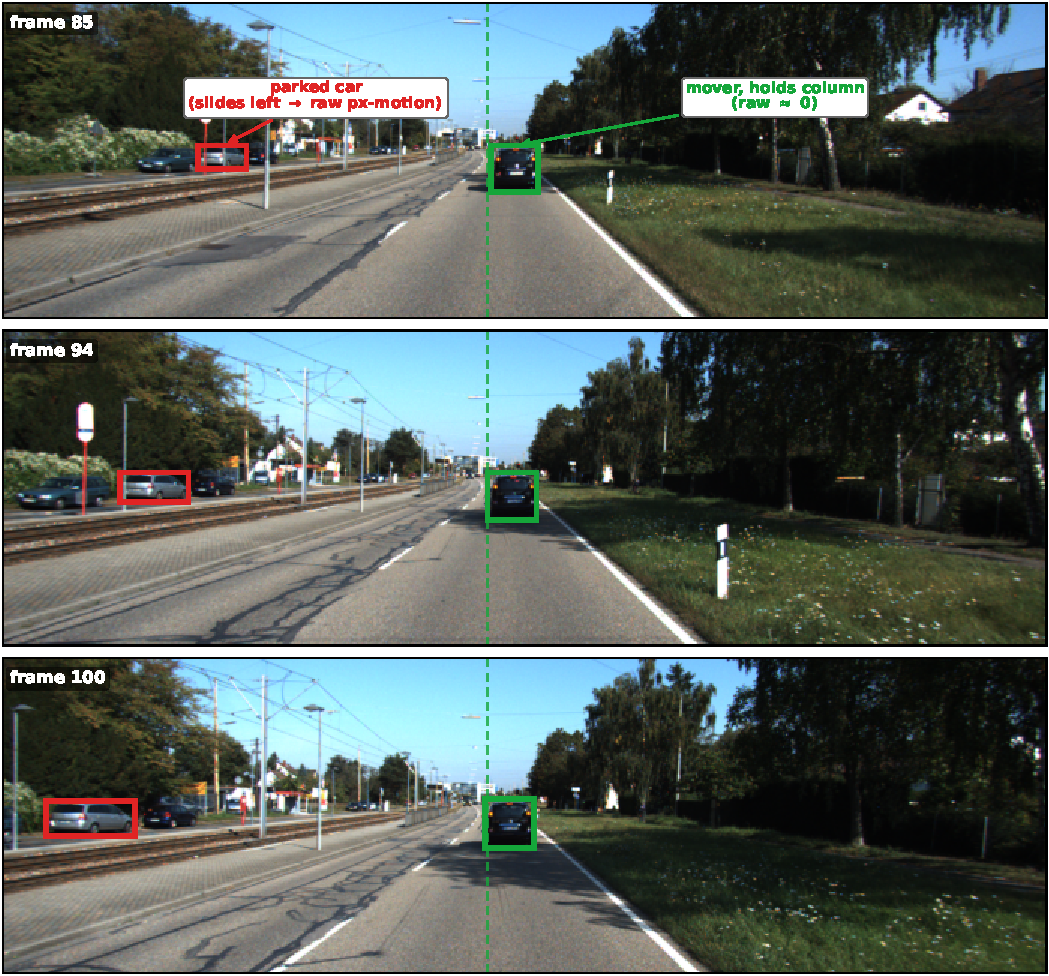
\includegraphics[width=\linewidth]{figures/qualitative.pdf}
  \caption{\DIFdelbeginFL \textbf{\DIFdelFL{Real recovery under camera ego-motion}} %DIFAUXCMD
\DIFdelFL{on ``moving cars'' (Refer-KITTI seq 0005, frames 85/94/100 of a forward-driving clip; the green car moves, the red car is parked). The dashed line marks the mover's image column. }\textbf{\DIFdelFL{Red:}} %DIFAUXCMD
\DIFdelFL{the parked car's centroid slides left as the camera passes it (center-$x$ $261\!\to\!104$\,px), so the camera-naive host scores it ``moving'' (false positive), yet its ego-compensated residual is near zero and the module restores it to static. }\textbf{\DIFdelFL{Green:}} %DIFAUXCMD
\DIFdelFL{the moving car holds its column (center-$x$ ${\approx}605$, ${<}1$\,px/frame), so the host misses it (false negative), but its nonzero residual --- unlike the static background --- recovers it as moving. Both errors flip from the same host logit through the additive correction.}\DIFdelendFL \DIFaddbeginFL \DIFaddFL{\textcolor{red}{``Moving cars'' (Refer-KITTI seq 0005). The parked car (red) sweeps across the image as the camera passes, while the moving car (green) barely shifts. Raw image motion misclassifies both; the ego-compensated residual recovers both from the same host score.}}\DIFaddendFL }
  \label{fig:qual}
\end{figure}

Figure~\ref{fig:qual} illustrates this behavior using a real example. The parked car moves across the image because of camera motion, while the moving car remains at nearly the same image location. Without ego-motion compensation, these two cases are easily confused because they have similar image-plane motion. After compensating for camera motion, the parked car has nearly zero residual motion, while the moving car retains nonzero residual motion. This allows GMC-Link to correctly distinguish between stationary and moving objects.

\DIFdelbegin \DIFdel{Finally, the complete module runs at $68$ FPS (median $14.8$\,ms/frame, excluding host inference), indicating that the proposed module can be integrated into existing RMOT frameworks with low computational overhead.
}%DIFDELCMD < 

%DIFDELCMD < %%%
\DIFdelend \section{Conclusion and Limitations}
\label{sec:conclusion}
GMC-Link is a decision-level plug-in module that improves motion grounding in referring multi-object tracking without modifying the detector, tracker, or appearance-language matching model. By compensating for camera motion and aligning residual motion with language descriptions, the proposed module helps distinguish object motion from camera-induced motion. \DIFdelbegin \DIFdel{Experimental results on Refer-KITTI show that GMC-Link improves moving-class HOTA in the evaluated host--split settings while maintaining competitive pooled HOTA, suggesting that it can enhance motion understanding without sacrificing overall tracking performance.
}\DIFdelend \DIFaddbegin \DIFadd{\textcolor{red}{Road-region background correspondences provide a geometric reference for estimating camera motion in driver-view driving scenes, after which the residual motion is aligned with language and integrated through late fusion with host-specific weights. On Refer-KITTI, pooled HOTA improves in all three evaluated host settings. For movement-related expressions, the largest gain is observed on iKUN ($+7.08\pm0.65$), and the ablation results show improvements in both MOVING and STATIC HOTA for the full module.}
}\DIFaddend 

Despite these promising results, several limitations remain. First, \DIFdelbegin \DIFdel{the proposed camera motion compensation relies on ORB and RANSAC, which estimate a single homography and may become less accurate in scenes with strong parallax or large non-planar motion}\DIFdelend \DIFaddbegin \DIFadd{\textcolor{red}{the road-plane homography assumes a flat ground, and falls back to the global estimate, which is less accurate, when it isn't}}\DIFaddend . Second, \DIFdelbegin \DIFdel{the fusion weight $\alpha$ is host-specific and needs to be selected for each host model. }\DIFdelend \DIFaddbegin \DIFadd{\textcolor{red}{a keyword classifier decides which weight an expression receives. Therefore, a misread expression gets the incorrect fusion weight: $14$ of the $126$ direction expressions in Refer-KITTI V1 are treated as appearance}. Third, \textcolor{red}{two weights do not help every host. On both FlexHook settings the leave-one-sequence-out procedure selects a single weight}. }\DIFaddend Finally, our experiments are conducted on two RMOT frameworks \DIFaddbegin \DIFadd{and the Refer-KITTI benchmarks}\DIFaddend , and additional evaluations on more host architectures and datasets are needed to further validate the generality of the proposed approach.

In future work, we plan to investigate more robust camera motion estimation methods and richer motion features that can better handle complex dynamic scenes. We also hope to evaluate GMC-Link on a broader range of referring multi-object tracking frameworks to further improve its generalization.

% References should be produced using the bibtex program from suitable
% BiBTeX files (here: strings, refs, manuals). The IEEEbib.bst bibliography
% style file from IEEE produces unsorted bibliography list.
% -------------------------------------------------------------------------
\bibliographystyle{IEEEbib}
\bibliography{refs}

\end{document}
